\section{Architecture}
\label{sec:arch}

\begin{figure*}[t]
\centering
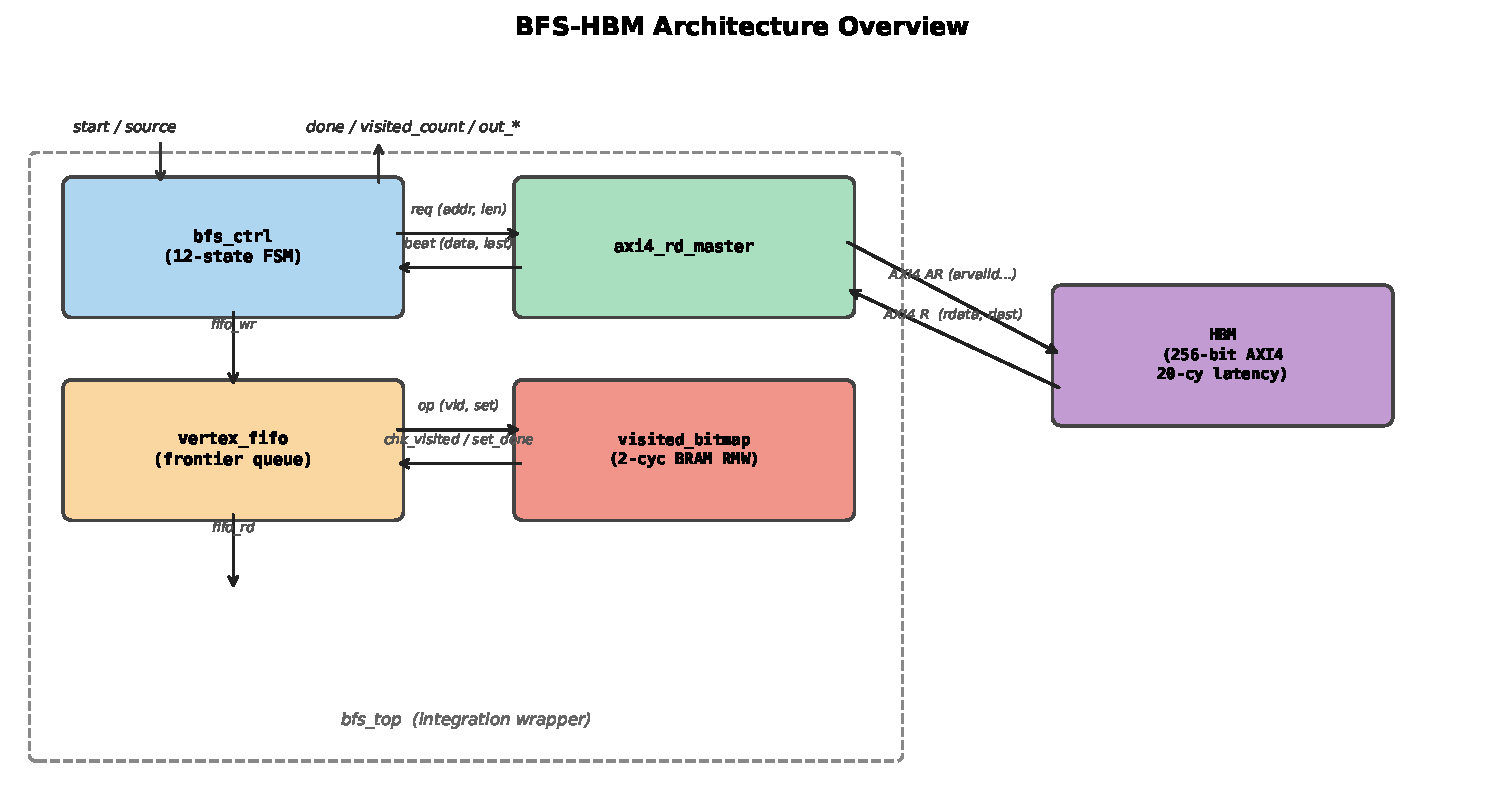
\includegraphics[width=0.9\textwidth]{figures/arch_overview.pdf}
\caption{BFS-HBM top-level architecture. Arrows show data flow; signal bundles are
labeled with width. The visited bitmap is the throughput bottleneck: its 2-cycle
RMW latency sets the upper bound on edge processing rate.}
\label{fig:arch}
\end{figure*}

Figure~\ref{fig:arch} shows the top-level module hierarchy. BFS-HBM decomposes into
five modules with well-defined, decoupled interfaces:

\begin{enumerate}[leftmargin=*,itemsep=3pt]
\item \textbf{\texttt{bfs\_ctrl}}: the traversal FSM. Orchestrates all other modules.
  Issues AXI4 read requests, processes incoming beats, drives the visited bitmap,
  and enqueues discovered vertices into the frontier FIFO.
\item \textbf{\texttt{axi4\_rd\_master}}: the AXI4 AR/R channel manager.
  Translates \texttt{(addr, len)} requests from \texttt{bfs\_ctrl} into compliant
  AXI4 transactions and presents incoming beats as a simple \texttt{(data, last)} stream.
\item \textbf{\texttt{vertex\_fifo}}: a synchronous FIFO storing frontier entries as
  packed $(\mathit{level}[15:0], \mathit{vid}[\mathit{VERTEX\_W}-1:0])$ words.
  Depth parameterized by \texttt{FIFO\_DEPTH} (default 2048).
\item \textbf{\texttt{visited\_bitmap}}: a 2-cycle BRAM-backed read-modify-write unit.
  Stores one bit per vertex; supports check (read) and set (RMW) operations on a
  unified request port.
\item \textbf{\texttt{bfs\_top}}: the integration wrapper. Instantiates all four
  modules and connects internal wires. Exposes the AXI4 read interface, the BFS
  control interface (\texttt{start}, \texttt{source}, \texttt{done}),
  and a discovery output stream (\texttt{out\_valid}, \texttt{out\_vid},
  \texttt{out\_level}).
\end{enumerate}

\subsection{Traversal State Machine}

\texttt{bfs\_ctrl} implements a 12-state Moore FSM. Table~\ref{tab:states} describes
each state and its exit condition.

\begin{table}[h]
\centering
\caption{BFS-HBM FSM states.}
\label{tab:states}
\small
\begin{tabular}{@{}lp{5.2cm}@{}}
\toprule
State & Function \\
\midrule
\textsc{Idle}       & Wait for \texttt{start} assertion. \\
\textsc{Init}       & Issue bitmap set for source vertex; enqueue source at level 0.
                       Assert \texttt{out\_valid} for source discovery. \\
\textsc{Dequeue}    & Pop frontier head into \texttt{cur\_vid}, \texttt{cur\_level}.
                       Transition to \textsc{Done} if FIFO empty. \\
\textsc{FetchPtr}   & Issue AXI4 read for \texttt{row\_ptr[cur\_vid]} (1-beat burst). \\
\textsc{WaitPtr}    & Accept incoming beat; latch \texttt{edge\_start}~(bits~31:0)
                       and \texttt{edge\_end}~(bits~63:32). \\
\textsc{CheckEdges} & Compute \texttt{edge\_remaining}. Skip to \textsc{Dequeue}
                       if vertex is a leaf ($\mathit{edge\_end} = \mathit{edge\_start}$). \\
\textsc{IssueEdges} & Issue AXI4 burst read for
                       \texttt{col\_idx[edge\_start..edge\_end-1]}. \\
\textsc{RecvBeat}   & Latch incoming 256-bit beat into 8-entry beat buffer. \\
\textsc{ScatterRd}  & Issue bitmap check for \texttt{beat\_buf[beat\_idx]}. \\
\textsc{ScatterChk} & Evaluate check result.
                       If unvisited: issue bitmap set, assert \texttt{fifo\_wr\_valid}
                       and \texttt{out\_valid}. \\
\textsc{NextEdge}   & Advance \texttt{beat\_idx} or fetch next beat. \\
\textsc{Done}       & Hold until reset. \\
\bottomrule
\end{tabular}
\end{table}

\subsection{Memory Layout and Single-Transaction Row Pointer Fetch}

A key architectural decision is the placement of \texttt{row\_ptr} and \texttt{col\_idx}
in HBM address space. \texttt{row\_ptr} is stored at \texttt{ROW\_PTR\_BASE}
(byte 0 by default); \texttt{col\_idx} at \texttt{COL\_IDX\_BASE} (1~MB offset).
Both arrays use 4-byte (32-bit) elements.

To expand vertex $v$, the FSM needs both $\mathit{row\_ptr}[v]$ and
$\mathit{row\_ptr}[v+1]$. These are at byte addresses
$\mathit{ROW\_PTR\_BASE} + 4v$ and $\mathit{ROW\_PTR\_BASE} + 4v + 4$ respectively.
Since a 256-bit HBM beat delivers 32 bytes, both values arrive in the low 64 bits of
a single beat (\texttt{arlen=0}, single-beat transaction):

\begin{equation}
\mathit{edge\_start} = \mathit{beat}[31:0], \quad
\mathit{edge\_end}   = \mathit{beat}[63:32]
\label{eq:ptr_unpack}
\end{equation}

This eliminates what would otherwise be a second AXI round trip per vertex,
saving approximately $T_\text{access}$ cycles per vertex expanded.

\subsection{Beat Buffer and Neighbor Processing}

With \texttt{AXI\_DATA\_W = 256} and 32-bit vertex IDs:
\begin{equation}
\mathit{VERTS\_PER\_BEAT} = \frac{256}{32} = 8
\end{equation}

The \textsc{RecvBeat} state latches an incoming 256-bit beat into an 8-entry
32-bit register array (\texttt{beat\_buf}). The FSM then iterates sequentially
through all 8 entries in the scatter loop (\textsc{ScatterRd} $\to$
\textsc{ScatterChk} $\to$ \textsc{NextEdge}), processing one neighbor per 2--3
cycles. When all entries are consumed, the FSM re-enters \textsc{RecvBeat} for the
next beat of the burst, or returns to \textsc{Dequeue} when all edges are processed.

\subsection{Discovery Output Stream}

The \texttt{(out\_valid, out\_vid, out\_level)} stream reports each newly discovered
vertex at the cycle \texttt{bm\_set\_done} fires for that vertex. This stream is
valid in both \textsc{Init} (source vertex at level 0) and \textsc{ScatterChk}
(each unvisited neighbor at \texttt{cur\_level + 1}). Downstream logic may use this
stream for result capture, depth limiting, or further workload-specific processing.
